
\documentclass[fleqn,addpoints]{exam}

\usepackage{graphicx}
\usepackage{booktabs}
\usepackage{float}
\usepackage{amsmath}
\usepackage{cancel}
\usepackage{polynom}
\usepackage{caption}
\usepackage{mdwlist}

\newcommand{\degree}{\ensuremath{^\circ}} 

\printanswers

\ifprintanswers 
\usepackage{2in1, lscape} 
\fi

\title{Math 115 \\ Homework 21}
\date{May 3, 2011}

\begin{document}

\maketitle

% \begin{figure}[H]
%   \centering
%   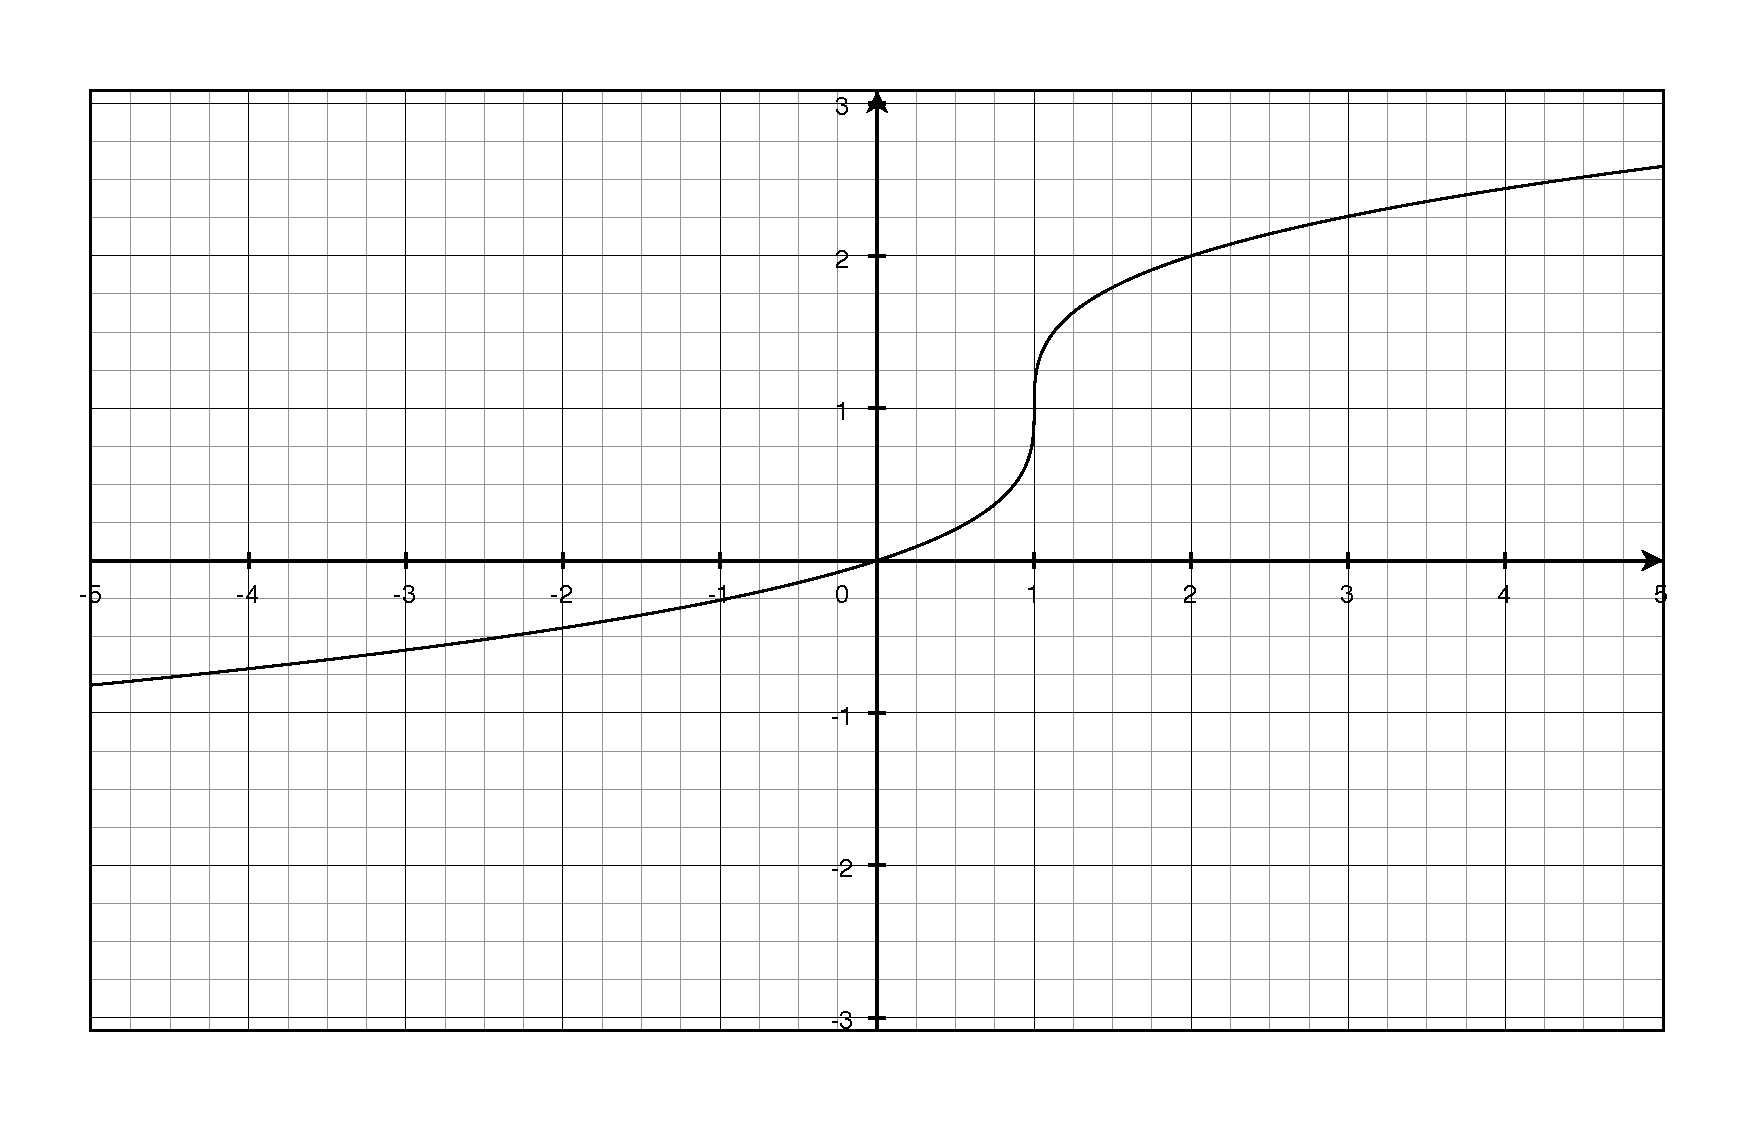
\includegraphics[scale=.3]{question7.eps}
%   \caption*{Question 7}
% \end{figure}

\ifprintanswers
\else
\section{Homework}
\begin{itemize*}
  \item pp 377-380: 1-2, 8-12, 17-18, 21-22, 37-38, 47-60, 62-65, 71-76
  \item pp 387-389: 3-6, 11-18, 26-27, 31-35, 41-42, 45-46, 55-58, 69-70, 86-90, 92, 95-96
\end{itemize*}

% 365 points possible

\fi

\section{Extra Credit}

An airplane is flying at an elevation of 5000 feet directly above a straight highway.  Two people are driving cars on
the highway on opposite sides of the plane.  The angle of depression to one car is $30 \degree$ and the angle of
depression to the other car is $45 \degree$.  How far apart are the cars?

\begin{solution}
If $d$ is the distance on the ground from the car to the point on the ground just below the airplane.

\begin{align*}
  \tan \theta &= \frac{5000}{d} \\
  d &= \frac{5000}{\tan \theta} \\
  d &= 5000 \cot \theta \\
\end{align*}

The total distance between the two cars is:
\[
  5000 \cot 30 + 5000 \cot 45 = 13,660 \text{ ft}
\]

\end{solution}

\ifprintanswers
\section{Pages 377-380}

\begin{description}

\item[1]
The missing side is: 
\[
  \sqrt{6^2 + 8^2} = \sqrt{100} = 10
\]

\begin{tabular}{cccccc}
\toprule
sin & cos & tan & csc & sec & cot \\
\midrule
  $\dfrac{3}{5}$ &  $\dfrac{4}{5}$ & $\dfrac{3}{4}$ & $\dfrac{5}{3}$ & $\dfrac{5}{4}$ & $\dfrac{4}{3}$ \\
\bottomrule
\end{tabular}

\item[2]
The missing side is:
\begin{align*}
  a^2 + 5^2 &= 13^2 \\
  a &= \sqrt{169-25} \\
  a &= \sqrt{144} \\
  a &= 12 \\
\end{align*}

\begin{tabular}{cccccc}
\toprule
sin & cos & tan & csc & sec & cot \\
\midrule
  $\dfrac{5}{13}$ &  $\dfrac{12}{13}$ & $\dfrac{5}{12}$ & $\dfrac{13}{5}$ & $\dfrac{13}{12}$ & $\dfrac{12}{5}$ \\
\bottomrule
\end{tabular}

\item[8]
The values are the same because the triangles are similar so the ratios of all the sides are the same.  The length of
the hypotenuse of the smaller triangle is $c = \sqrt{1^2 + 2^2} = \sqrt{5}$

\begin{tabular}{cccccc}
\toprule
sin & cos & tan & csc & sec & cot \\
\midrule
  $\dfrac{\sqrt{5}}{5}$ &  $\dfrac{2 \sqrt{5}}{5}$ & $\dfrac{1}{2}$ & $\sqrt{5}$ & $\dfrac{\sqrt{5}}{2}$ & $2$ \\
\bottomrule
\end{tabular}

\item[9]
\begin{align*}
  a^2 + 3^2 &= 4^2 \\
  a^2 + 9 &= 16 \\
  a^2 &= 7 \\
  a &= \sqrt{7} \\
\end{align*}

\begin{tabular}{cccccc}
\toprule
sin & cos & tan & csc & sec & cot \\
\midrule
  $\dfrac{3}{4}$ &  $\dfrac{\sqrt{7}}{4}$ & $\dfrac{3 \sqrt{7}}{7}$ & $\dfrac{4}{3}$ & $\dfrac{4 \sqrt{7}}{7}$ & $\dfrac{\sqrt{7}}{3}$ \\
\bottomrule
\end{tabular}

\item[10]
\begin{align*}
  a^2 + 5^2 &= 7^2 \\
  a^2 + 25 &= 49 \\
  a^2 &= 24 \\
  a &= 2\sqrt{6} \\
\end{align*}

\begin{tabular}{cccccc}
\toprule
sin & cos & tan & csc & sec & cot \\
\midrule
  $\dfrac{2 \sqrt{6}}{7}$ &  $\dfrac{5}{7}$ & $\dfrac{2 \sqrt{6}}{5}$ & $\dfrac{7 \sqrt{6}}{12}$ & $\dfrac{7}{5}$ & $\dfrac{5 \sqrt{6}}{12}$ \\
\bottomrule
\end{tabular}

\item[11]
\begin{align*}
  a^2 + 1^2 &= 2^2 \\
  a^2 + 1 &= 4 \\
  a^2 &= 3 \\
  a &= \sqrt{3} \\
\end{align*}

\begin{tabular}{cccccc}
\toprule
sin & cos & tan & csc & sec & cot \\
\midrule
  $\dfrac{\sqrt{3}}{2}$ &  $\dfrac{1}{2}$ & $\sqrt{3}$ & $\dfrac{2 \sqrt{3}}{3}$ & $2$ & $\dfrac{\sqrt{3}}{3}$ \\
\bottomrule
\end{tabular}

\item[12]

\begin{tabular}{cccccc}
\toprule
sin & cos & tan & csc & sec & cot \\
\midrule
  $\dfrac{\sqrt{26}}{26}$ &  $\dfrac{5 \sqrt{26}}{26}$ & $\dfrac{1}{5}$ & $\sqrt{26}$ & $\dfrac{\sqrt{26}}{5}$ & $5$ \\
\bottomrule
\end{tabular}

\item[17]
\begin{description}
\item[a] $\tan 60 \degree = \sqrt{3}$

\item[b] $\sin 30 \degree = \dfrac{1}{2}$

\item[c] $\cos 30 \degree = \dfrac{\sqrt{3}}{2}$

\item[d] $\cot 60 \degree = \dfrac{\sqrt{3}}{3}$

\end{description}

\item[18]
\begin{description}
\item[a] $\csc 30 \degree = 2$

\item[b] $\cot 60 \degree = \dfrac{\sqrt{3}}{3}$

\item[c] $\cos 30 \degree = \dfrac{\sqrt{3}}{2}$

\item[d] $\cot 30 \degree = \sqrt{3}$

\end{description}

\item[21]
\begin{align*}
  a^2 + 1^2 &= 3^2 \\
  a^2 + 1 &= 9 \\
  a^2 &= 8 \\
  a &= 2 \sqrt{2} \\
\end{align*}

\begin{tabular}{cccccc}
\toprule
sin & cos & tan & csc & sec & cot \\
\midrule
  $\dfrac{2 \sqrt{2}}{3}$ &  $\dfrac{1}{3}$ & $\dfrac{2 \sqrt{2}}{3}$ & $\dfrac{\sqrt{2}}{4}$ & $3$ & $\dfrac{3 \sqrt{2}}{4}$ \\
\bottomrule
\end{tabular}

 \item[22]
\begin{align*}
  5^2 + 1^2 &= c^2 \\
  25 + 1 &= c^2 \\
  c &= \sqrt{26} \\
\end{align*}

\begin{tabular}{cccccc}
\toprule
sin & cos & tan & csc & sec & cot \\
\midrule
  $\dfrac{5 \sqrt{26}}{26}$ &  $\dfrac{\sqrt{26}}{26}$ & $5$ & $\dfrac{\sqrt{26}}{5}$ & $\sqrt{26}$ & $\dfrac{1}{5}$ \\
\bottomrule
\end{tabular}

\item[37]
\begin{description}
\item[a]
\begin{align*}
  \sin \theta &= \frac{1}{2} \\
  \theta &= \frac{\pi}{6} \\  
  \theta &= 30 \degree \\
\end{align*}

\item[b]
\begin{align*}
  \csc \theta &= 2 \\
  \sin \theta &= \frac{1}{2} \\
  \theta &= \frac{\pi}{6} \\
  \theta &= 30 \degree \\
\end{align*}

\end{description}

\item[38]
\begin{description}
\item[a]
\begin{align*}
  \cos \theta &= \frac{\sqrt{2}}{2} \\
  \theta &= \frac{\pi}{4} \\
  \theta &= 45 \degree \\
\end{align*}

\item[b]
\begin{align*}
  \tan \theta &= 1 \\
  \theta &= \frac{\pi}{4} \\
  \theta &= 45 \degree \\
\end{align*}

\end{description}

\item[47]
\begin{align*}
  \tan 30 \degree &= \frac{30}{x} \\
   x &= \frac{30}{\tan 30 \degree} \\
   &= 30 \sqrt{3} \\
   & \approx 52.0 \\
\end{align*}

\item[48]
\begin{align*}
  \sin 60 \degree &= \frac{y}{18} \\
  y &= 18 \sin 60 \degree \\
   &= 18 \frac{\sqrt{3}}{2} \\
   &= 9 \sqrt{3} \\
   &\approx 15.6 \\
\end{align*}

\item[49]
\begin{align*}
  \tan 60 \degree &= \frac{32}{x} \\
  x &= \frac{32}{\tan 60 \degree} \\
   &= \frac{32 \sqrt{3}}{3} \\
   & \approx 18.48 \\
\end{align*}

\item[50]
\begin{align*}
  \sin 45 \degree &= \frac{20}{r} \\
  r &= \frac{20}{\sin 45 \degree} \\
   &= 20 \sqrt{2} \\
   & \approx 28.28 \\
\end{align*}

\item[51]
\[
  \tan \theta \cot \theta 
  = \frac{\cancel{\sin \theta}}{\cancel{\cos \theta}} \cdot \frac{\cancel{\cos \theta}}{\cancel{\sin \theta}} = 1 
\]

\item[52]
\[
  \cos \theta \sec \theta = \cancel{\cos \theta} \cdot \frac{1}{\cancel{\cos \theta}} = 1
\]

\item[53]
\[
  \tan \alpha \cos \alpha = \frac{\sin \alpha}{\cancel{\cos \alpha}} \cdot \cancel{\cos \alpha} = \sin \alpha
\]

\item[54]
\[
  \cot \alpha \sin \alpha = \frac{\cos \alpha}{\cancel{\sin \alpha}} \cdot \cancel{\sin \alpha} = \cos \alpha
\]

\item[55]
\[
  (1 + \cos \theta)(1 - \cos \theta) = 1 - \cos^2 \theta = \sin^2 \theta
\]

\item[56]
\[
  (1 + \sin \theta)(1 - \sin \theta) = 1 - \sin^2 \theta = \cos^2 \theta
\]

\item[57]
\[
  (\sec \theta + \tan \theta)(\sec \theta - \tan \theta) = \sec^2 \theta - \tan^2 \theta = 1 + \tan^2 \theta - \tan^2 \theta = 1
\]

\item[58]
\[
  \sin^2 \theta - \cos^2 \theta = \sin^2 \theta - (1 - \sin^2 \theta) = 2 \sin^2 \theta - 1
\]

\item[59]
\begin{align*}
  \frac{\sin \theta}{\cos \theta} + \frac{\cos \theta}{\sin \theta} &= \frac{\sin^2 \theta + \cos^2 \theta}{\sin \theta \cos \theta} \\
  &= \frac{1}{\sin \theta \cos \theta} \\
  &= \csc \theta \sec \theta \\
\end{align*}

\item[60]
\begin{align*}
  \frac{\tan \beta + \cot \beta}{\tan \beta} &= \frac{\cancel{\tan \beta}}{\cancel{\tan \beta}} + \frac{\cot \beta}{\tan \beta} \\
  &= 1 + \frac{\cos \beta}{\sin \beta} \cdot \frac{\cos \beta}{\sin \beta} \\
  &= 1 + \frac{\cos^2 \beta}{\sin^2 \beta} \\
  &= 1 + \cot^2 \beta \\
  &= \csc^2 \theta
\end{align*}

\item[62]

If $\theta$ is the angle made by the light and the street:
\begin{align*}
  \tan \theta &= \frac{h}{30} \\
  \tan \theta &= \frac{6}{10} \\
  \frac{6}{10} &= \frac{h}{30} \\
  \frac{3}{5} &= \frac{h}{30} \\
  h &= 18 \\
\end{align*}

\item[63]
\begin{align*}
  \sin 85 \degree &= \frac{h}{20} \\
  h &= 20 \sin 85 \degree \\
  h &\approx 19.9 \text{ meter} \\
\end{align*}

\item[64]
\begin{align*}
  \tan 54 \degree &= \frac{w}{100} \\
  w &= 100 \tan 54 \degree \\
  w &\approx 138 \text{ ft} \\
\end{align*}

\item[65]
\begin{align*}
  \tan 4 \degree &= \frac{40}{x} \\
  x &= \frac{40}{\tan 4 \degree} \\
  h &\approx 572 \text{ ft} \\
\end{align*}

\item[71]
true since $\csc x = \dfrac{1}{\sin x}$

\item[72]
true since:
\begin{align*}
  \sec x &= \frac{1}{\cos x} \\
  &= \frac{1}{\sin (90 \degree - x)} \\
  &= \csc(90 \degree - x) \\
\end{align*}

\item[73]
false: $\dfrac{\sqrt{2}}{2} + \dfrac{\sqrt{2}}{2} = \sqrt{2} \neq 1$

\item[74]
true since: $\cot^2 x + 1 = \csc^2 x$

\item[75]
false since: $\dfrac{1/2}{\sqrt{3}/2} = \dfrac{1}{2} \cdot \dfrac{2}{\sqrt{3}} = \dfrac{\sqrt{3}}{3} \neq sin 2 \degree$

\item[76]
false

\end{description}

\section{Pages 387-389}
\begin{description}

\item[3]
\begin{description}
\item[a]
\[
  r = \sqrt{\left( -\sqrt{3} \right)^2 + (-1)^2} = \sqrt{4} = 2
\]

\begin{tabular}{cccccc}
\toprule
sin & cos & tan & csc & sec & cot \\
\midrule
  $-\dfrac{1}{2}$ &  $- \dfrac{\sqrt{3}}{2}$ & $\dfrac{\sqrt{3}}{3}$ & $-2$ & $-\dfrac{2 \sqrt{3}}{3}$ & $\sqrt{3}$ \\
\bottomrule
\end{tabular}

\item[b]
\[
  r = \sqrt{(-4)^2 + 1^2} = \sqrt{17}
\]

\begin{tabular}{cccccc}
\toprule
sin & cos & tan & csc & sec & cot \\
\midrule
  $\dfrac{\sqrt{17}}{5}$ &  $- \dfrac{4\sqrt{17}}{5}$ & $-\dfrac{1}{4}$ & $\sqrt{17}$ & $-\dfrac{\sqrt{17}}{4}$ & $-4$ \\
\bottomrule
\end{tabular}


\end{description}

\item[4]
\begin{description}
\item[a]
\[
  r = \sqrt{3^2 + 1^2} = \sqrt{10}
\]

\begin{tabular}{cccccc}
\toprule
sin & cos & tan & csc & sec & cot \\
\midrule
  $\dfrac{\sqrt{10}}{10}$ &  $\dfrac{3 \sqrt{10}}{10}$ & $\dfrac{1}{3}$ & $\sqrt{10}$ & $\dfrac{\sqrt{10}}{3}$ & $3$ \\
\bottomrule
\end{tabular}

\item[b]
\[
  r = \sqrt{4^2 + (-4)^2} = \sqrt{32} = 4 \sqrt{2}
\]

The angle is $-\dfrac{\pi}{4}$.

\begin{tabular}{cccccc}
\toprule
sin & cos & tan & csc & sec & cot \\
\midrule
  $-\dfrac{\sqrt{2}}{2}$ &  $\dfrac{\sqrt{2}}{2}$ & $-1$ & $- \sqrt{2}$ & $\sqrt{2}$ & $-1$ \\
\bottomrule
\end{tabular}

\end{description}

\item[5]
\[
  r = \sqrt{7^2 + 24^2} = \sqrt{625} = 25
\]

\begin{tabular}{cccccc}
\toprule
sin & cos & tan & csc & sec & cot \\
\midrule
  $\dfrac{24}{25}$ &  $\dfrac{7}{25}$ & $\dfrac{24}{7}$ & $\dfrac{25}{24}$ & $\dfrac{25}{7}$ & $\dfrac{7}{24}$ \\
\bottomrule
\end{tabular}

\item[6]
\[
  r = \sqrt{8^2 + 15^2} = \sqrt{289} = 17
\]

\begin{tabular}{cccccc}
\toprule
sin & cos & tan & csc & sec & cot \\
\midrule
  $\dfrac{15}{17}$ &  $\dfrac{8}{17}$ & $\dfrac{15}{8}$ & $\dfrac{17}{15}$ & $\dfrac{17}{8}$ & $\dfrac{8}{15}$ \\
\bottomrule
\end{tabular}

\item[11] III
\item[12] I
\item[13] II
\item[14] IV

\item[15]
\begin{tabular}{cccccc}
\toprule
sin & cos & tan & csc & sec & cot \\
\midrule
  $\dfrac{3}{5}$ &  $- \dfrac{4}{5}$ & $- \dfrac{3}{4}$ & $\dfrac{5}{3}$ & $-\dfrac{5}{4}$ & $- \dfrac{4}{3}$ \\
\bottomrule
\end{tabular}

\item[16]
\begin{tabular}{cccccc}
\toprule
sin & cos & tan & csc & sec & cot \\
\midrule
  $-\dfrac{3}{5}$ &  $- \dfrac{4}{5}$ & $\dfrac{3}{4}$ & $-\dfrac{5}{3}$ & $-\dfrac{5}{4}$ & $\dfrac{4}{3}$ \\
\bottomrule
\end{tabular}

\item[17]
\begin{tabular}{cccccc}
\toprule
sin & cos & tan & csc & sec & cot \\
\midrule
  $-\dfrac{15}{17}$ &  $\dfrac{8}{17}$ & $- \dfrac{15}{8}$ & $-\dfrac{17}{15}$ & $\dfrac{17}{8}$ & $-\dfrac{8}{15}$ \\
\bottomrule
\end{tabular}

\item[18]
\begin{tabular}{cccccc}
\toprule
sin & cos & tan & csc & sec & cot \\
\midrule
  $-\dfrac{15}{17}$ &  $\dfrac{8}{17}$ & $- \dfrac{15}{8}$ & $-\dfrac{17}{15}$ & $\dfrac{17}{8}$ & $-\dfrac{8}{15}$ \\
\bottomrule
\end{tabular}

\item[22]
\begin{description}
\item[a] $\cot \beta = \frac{1}{5}$

\item[b] $\cot \beta = \dfrac{\sqrt{\sqrt{26}}}{26}$

\item[c] $\tan (90 - \beta) = \frac{1}{5}$

\item[d] $\csc \beta = \dfrac{\sqrt{26}}{5}$

\end{description}

\item[26]

Since the slope is $\dfrac{1}{3}$, the point $(-3, -1)$ is on the line in the right quadrant.  We can use this point to
find that the radius is: 
\[
  r = \sqrt{3^1 + 1^2} = \sqrt{10}
\]

\begin{tabular}{cccccc}
\toprule
sin & cos & tan & csc & sec & cot \\
\midrule
  $-\dfrac{\sqrt{10}}{10}$ &  $-\dfrac{3 \sqrt{10}}{10}$ & $\dfrac{1}{3}$ & $-\sqrt{10}$ & $-\dfrac{\sqrt{10}}{3}$ & $3$ \\
\bottomrule
\end{tabular}

\item[27]
\begin{align*}
  2x - y &= 0 \\
  y &= 2x \\
\end{align*}

Since the slope is $2$, the point $(1, 2)$ is on the line.  We can use this point to find that the radius is:
\[
  r = \sqrt{1^1 + 2^2} = \sqrt{5}
\]

\begin{tabular}{cccccc}
\toprule
sin & cos & tan & csc & sec & cot \\
\midrule
  $-\dfrac{2 \sqrt{5}}{5}$ & $-\dfrac{\sqrt{5}}{5}$ & $2$ & $- \dfrac{\sqrt{5}}{2}$ & $-\sqrt{5}$ & $\dfrac{1}{2}$ \\
\bottomrule
\end{tabular}

\item[31]
\[
  \sec \pi = \frac{1}{\cos \pi} = -1
\]

\item[32]
undefined

\item[33]
undefined

\item[34]
\[
  \tan \pi = 0
\]

\item[35]
\[
  \cot \frac{\pi}{2} = 0
\]


\item[45]
\[
  225 \degree - 180 \degree = 45 \degree
\]

The angle is in the third quadrant, so $\cos$ and $\sin$ are negative and $\tan$ is positive

\begin{tabular}{ccc}
\toprule
sin & cos & tan \\
\midrule
  $-\dfrac{\sqrt{2}}{2}$ & $-\dfrac{\sqrt{2}}{2}$ & $1$ \\
\bottomrule
\end{tabular}

\item[46]
\[
  360 \degree - 300 \degree = 60 \degree
\]

The angle is in the fourth quadrant, so $\cos$ is positive and $\sin$ and $\tan$ are negative.

\begin{tabular}{ccc}
\toprule
sin & cos & tan \\
\midrule
  $-\dfrac{\sqrt{3}}{2}$ & $\dfrac{1}{2}$ & $-\sqrt{3}$ \\
\bottomrule
\end{tabular}

\item[55]
\[
  \frac{12 \pi}{4} - \frac{11 \pi}{4} = \frac{\pi}{4}
\]

The angle is in the second quadrant, so $\cos$ and $\tan$ are negative and $\sin$ is positive.

\begin{tabular}{ccc}
\toprule
sin & cos & tan \\
\midrule
  $\dfrac{\sqrt{2}}{2}$ & $-\dfrac{\sqrt{2}}{2}$ & $-1$ \\
\bottomrule
\end{tabular}

\item[56]
\[
  \frac{10 \pi}{3} = 3 \pi + \frac{\pi}{3}
\]

The angle is in the third quadrant, so $\cos$ and $\sin$ are negative and $\tan$ is positive.

\begin{tabular}{ccc}
\toprule
sin & cos & tan \\
\midrule
  $-\dfrac{\sqrt{3}}{2}$ & $-\dfrac{1}{2}$ & $\sqrt{3}$ \\
\bottomrule
\end{tabular}

\item[57]

The reference angle is $\dfrac{\pi}{2}$.

\begin{tabular}{ccc}
\toprule
sin & cos & tan \\
\midrule
  $1$ & $0$ & undefined \\
\bottomrule
\end{tabular}

\item[58]
\[
  -\frac{25 \pi}{4} = -6 \pi - \frac{\pi}{4}
\]

The angle is in the fourth quadrant, so $\sin$ and $\tan$ are negative and $\cos$ is positive.

\begin{tabular}{ccc}
\toprule
sin & cos & tan \\
\midrule
  $-\dfrac{\sqrt{2}}{2}$ & $\dfrac{\sqrt{2}}{2}$ & $-1$ \\
\bottomrule
\end{tabular}

\item[69]
\begin{description}
\item[a]
\begin{align*}
  \theta &= \frac{\pi}{6} \\
  \theta &= \frac{5 \pi}{6} \\
  \theta &= 30 \degree \\
  \theta &= 150 \degree \\
\end{align*}

\item[b]
\begin{align*}
  \theta &= \frac{11 \pi}{6} \\
  \theta &= \frac{7 \pi}{3} \\
  \theta &= 330 \degree \\
  \theta &= 210 \degree \\
\end{align*}

\end{description}

\item[70]
\begin{description}
\item[a]
\begin{align*}
  \theta &= \frac{\pi}{4} \\
  \theta &= \frac{7 \pi}{4} \\
  \theta &= 45 \degree \\
  \theta &= 315 \degree \\
\end{align*}

\item[b]
\begin{align*}
  \theta &= \frac{5 \pi}{4} \\
  \theta &= \frac{3 \pi}{4} \\
  \theta &= 225 \degree \\
  \theta &= 315 \degree \\
\end{align*}

\end{description}

\item[86]
\begin{align*}
  \csc^2 \theta' &= 1 + (-3)^2 \\
  \csc^2 \theta' &= 10 \\
  \csc \theta' &= \sqrt{10} \\
  \sin \theta' &= \frac{\sqrt{10}}{10} \\
\end{align*}

Since $\theta$ is in the second quadrant, $\sin \theta = \dfrac{\sqrt{10}}{10}$

\item[87]
\begin{align*}
  \sec^2 \theta' &= 1 + \left( \frac{3}{2} \right)^2\\
  \sec^2 \theta' &= 1 + \frac{9}{4} \\
  \sec \theta' &=  \frac{\sqrt{13}}{2} \\
\end{align*}

Since $\theta$ is in the third quadrant, $\sec \theta = -\dfrac{\sqrt{13}}{2}$

\item[88]

\begin{align*}
  (-2)^2 &= 1 + \cot^2 \theta' \\
  4 &= 1 + \cot^2 \theta' \\
  \cot^2 \theta' &= 3 \\
  \cot \theta' &= \sqrt{3} \\
\end{align*}
Since $\theta$ is in the fourth quadrant, $\cot \theta = - \sqrt{3}$

\item[89]
\[
  \sec \theta = \frac{1}{\cos \theta} = \frac{8}{5}
\]

\item[90]
\begin{align*}
  \left( -\frac{9}{4} \right)^2 &= 1 + \tan^2 \theta' \\
  \frac{81}{16} &= 1 + \tan^2 \theta' \\
  \tan^2 \theta' &= \frac{65}{16} \\
  \tan \theta' &= \frac{\sqrt{65}}{4} \\
\end{align*}

Since $\theta$ is in the third quadrant, $\tan \theta = \dfrac{\sqrt{65}}{4}$.

\item[92]
.

\begin{tabular}{lcc}
\toprule
Date & $t$ & $S$ \\
\midrule
February 2001 & 2 & 27.7 \\
September 2001 & 9 & 25.6 \\
February 2002 & 14 & 32.7 \\
September 2002 & 21 & 27.7 \\
\bottomrule
\end{tabular}

\begin{figure}[H]
  \centering
  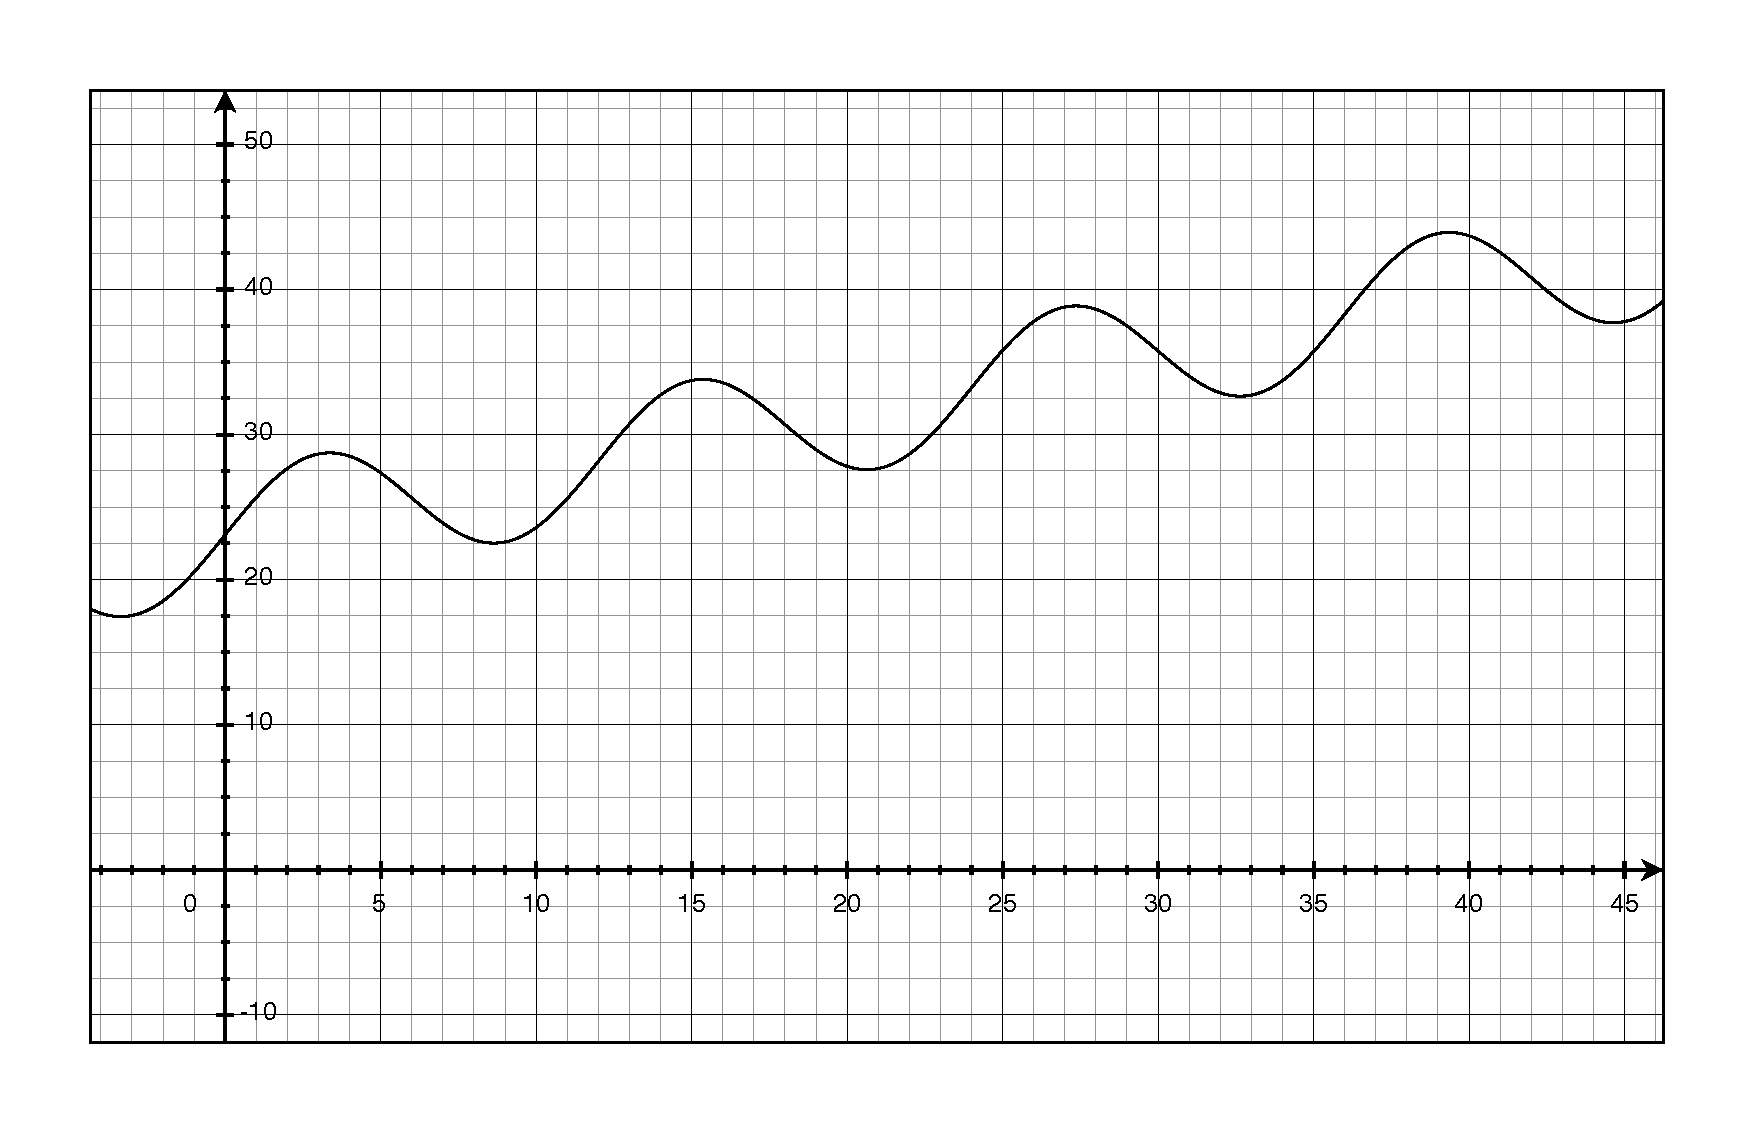
\includegraphics[scale=.3]{question92.eps}
  \caption*{Question 92}
\end{figure}

It looks like this company consistently sells a lot of stuff in the winter and doesn't sell much in the summer.  Maybe
they're selling snow shovels.  You can also see from the graph that they are consistently growing, on average, over time.

\item[95]

\[
  I = 5 e^{-2 \cdot 0.7} \sin 0.7 \approx 0.794
\]

\begin{figure}[H]
  \centering
  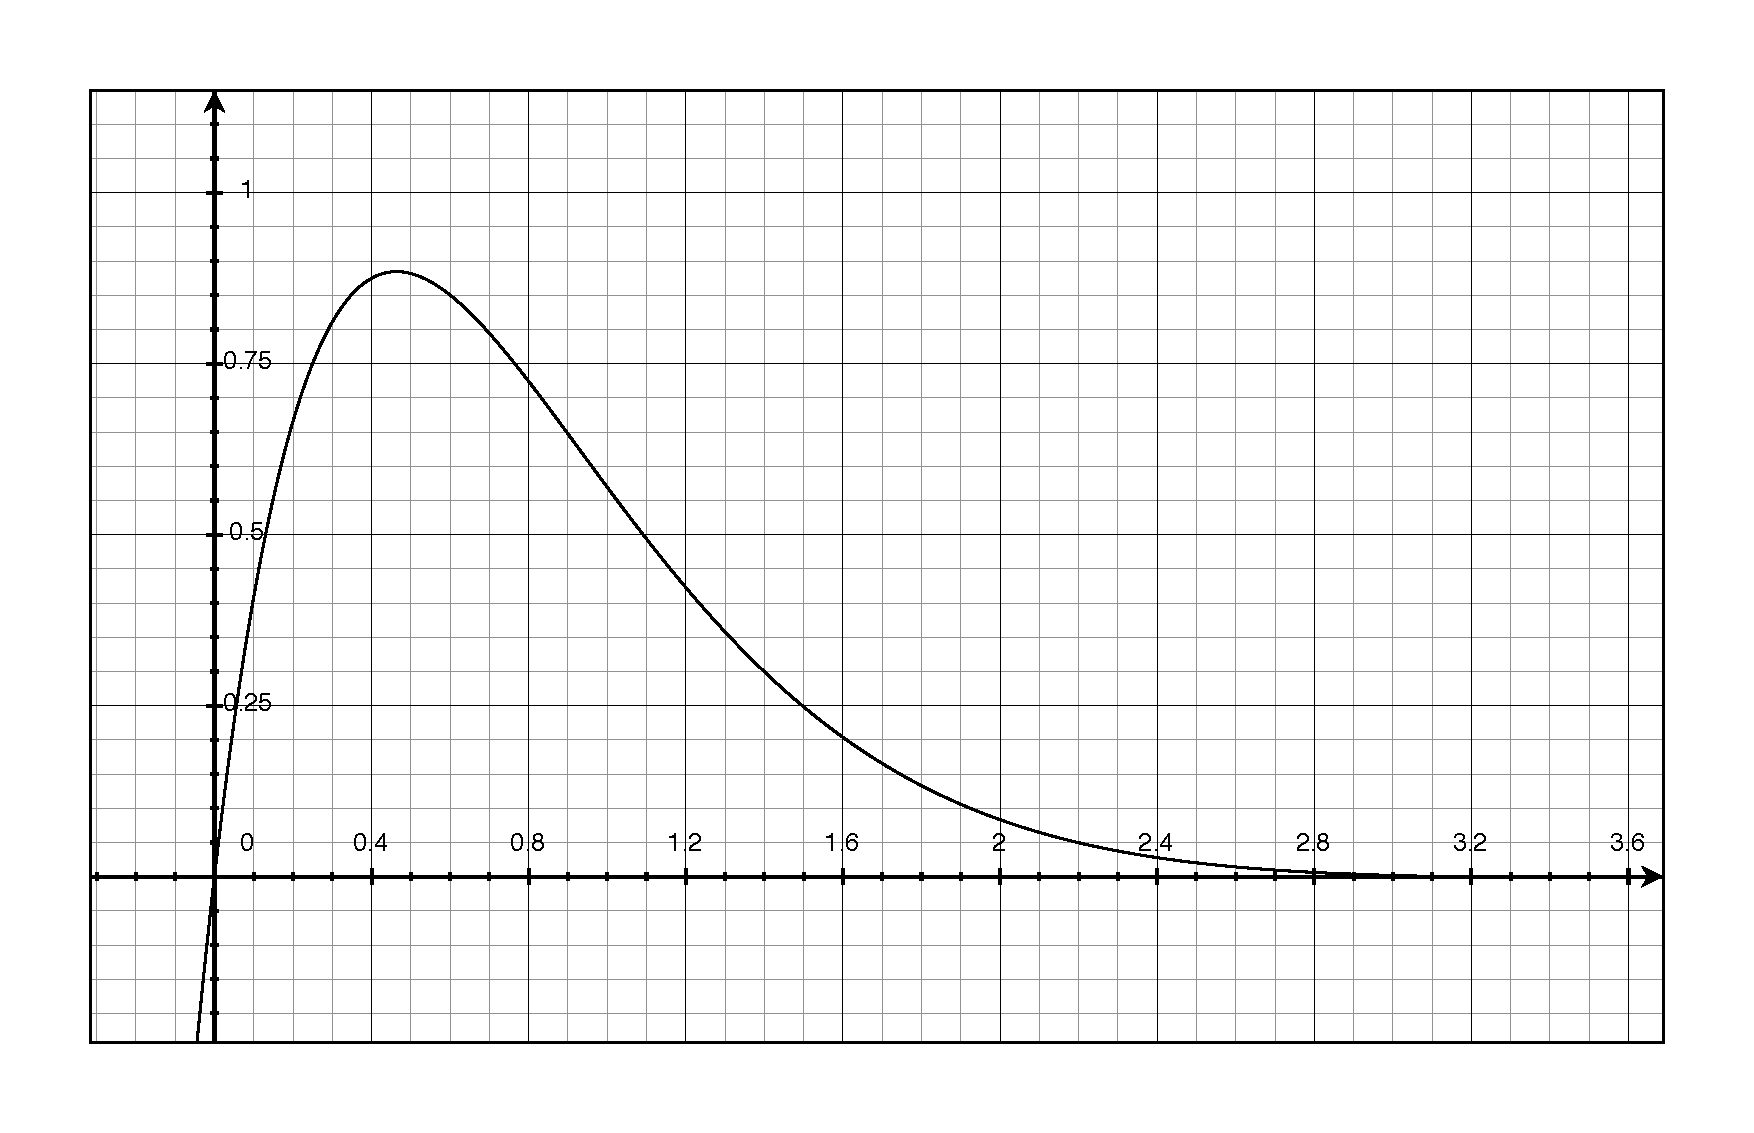
\includegraphics[scale=.3]{question95.eps}
  \caption*{Question 95}
\end{figure}

\item[96]

\begin{align*}
  \sin \theta &= \frac{6}{d} \\
  d &= \frac{6}{\sin \theta} \\
   &= 6 \sec \theta \\
\end{align*}

\begin{tabular}{cl}
\toprule
$\theta$ & $d$ \\
\midrule
$30 \degree$ & 12 miles   \\
$90 \degree$ & 6 miles   \\
$120 \degree$ & 6.9 miles   \\
\bottomrule
\end{tabular}


\end{description}

\else

\vspace{4 in}

\begin{em}
Everything is for sale, including men's souls. A man cannot understand the art he is studying if he only looks for the end
result without taking the time to delve deeply into the reasoning of the study.  There is no purpose in trying to
determine if one is better than another.  If anything is anything then everything is everything.
\end{em}

\vspace{.2 cm}
\hspace{1.5 cm} --Miyamoto Musashi, {\em The Book of Five Rings}

\fi

\end{document}

